\chapter{Algoritmo de sincronización y control de formaciones}
El algoritmo de sincronización y control de formaciones funciona de manera centralizada 


\subsection{Controlador del supervisor}
\subsection{Controlador de los agentes}
\subsection{Secuencia de ejecución del programa}


\chapter{Restauración del algoritmo desarrollado en fases previas}
La implementación en físico del algoritmo de sincronización y control de formaciones llevada a cabo por José Alejandro Rodríguez \cite{RodriguezJA_2023_tesis} se realizó en Webots con la versión 2023b. Esta es la misma versión que la utilizada en la fase actual. Además, se optó por utilizar Python 3.10 como lenguaje de programación para el controlador del supervisor y de los agentes ya que es una de las versiones más recientes de software, además que es la misma versión utilizada en la fase anterior. 

Por otro lado, en el Robotat se han realizado cambios en las conexiones con el servidor y los Pololu 3Pi+	por lo que se sería necesario un reajuste de parámetros.

En este capítulo se detallarán las modificaciones necesarias para la restauración del algoritmo y su correcta ejecución en simulaciones con Webots y en un entorno físico con el Robotat.


\section{Replicar simulaciones de Webots}

El primer paso de la restauración, fue recrear algunas simulaciones en Webots. Para esto, fue necesario instalar las siguientes librerías que no se encuentran dentro de la biblioteca estándar de Python:
\begin{itemize}
	\item Keyboard - versión 0.13.5
	\item NumPy - versión 1.23.2
\end{itemize}

Luego, se realizó la prueba del código para el controlador del supervisor y los agentes incluyendo sus respectivas funciones
\begin{itemize}
	\item Supervisor: Supervisor\_simulacion\_y\_fisico\_v4.py
	\item Agentes: pruebaMatrizDifeomorfismo.py
	\item Funciones algoritmo: funciones.py, funVel.py
\end{itemize} 

\subsection{Comunicación entre supervisor y agentes}
Al ejecutar una simulación, se encontró que dos agentes permanecen inmóviles durante todas las etapas del algoritmo, tal como se muestra en la Figura \ref{fig:delaygpu}.

\begin{figure}[H]
	\centering
	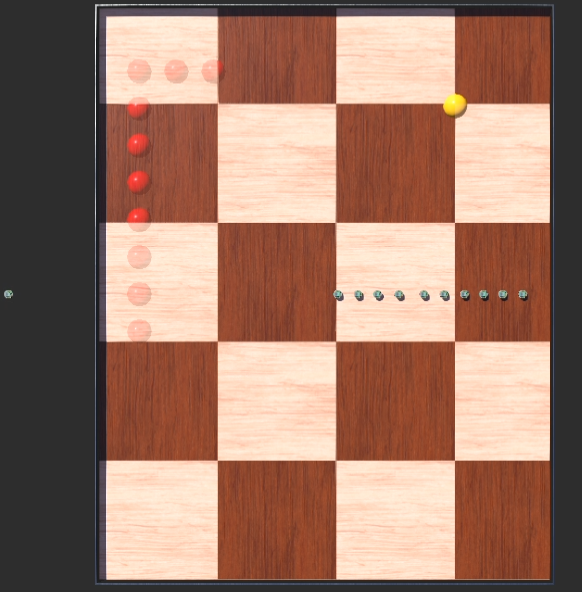
\includegraphics[width=0.30\textwidth]{delaygpu1.png}
	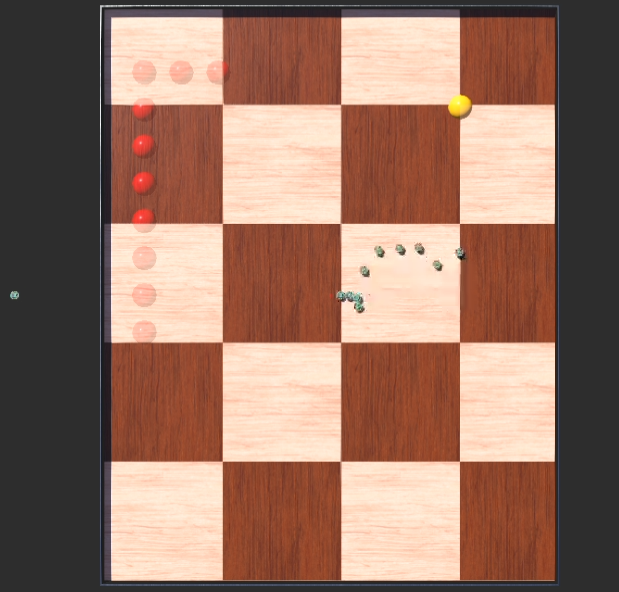
\includegraphics[width=0.30\textwidth]{delaygpu2.png}
	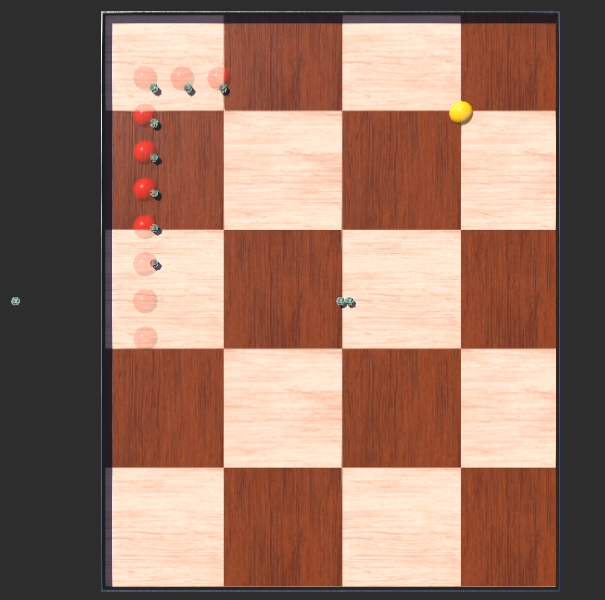
\includegraphics[width=0.30\textwidth]{delaygpu3.png}
	\caption{Ejecución de la primera simulación den Webots 2023b.}
	\label{fig:delaygpu}
\end{figure}

Esto se debe a que, actualmente, se está utilizando una computadora con mayor capacidad de procesamiento que la utilizada en la fase anterior. Esta capacidad de procesamiento radica en la velocidad de ejecución de los programas. 

Dado que la comunicación entre el supervisor y los agentes se realiza por medio de una memoria compartida y la velocidad de procesamiento es mayor, el controlador de los dos primeros agentes se ejecuta antes de que el espacio de memoria compartida se haya inicializado correctamente. Para solucionar el problema, en el controlador de los agentes, se agregó un tiempo de espera de 3 segundos antes de inicializar y acceder a la memoria compartida para asegurar que esta se cree correctamente.

%\subsection{Cambios en el entorno de simulación}
%En Webots 
%	Se cambió las medidas de la cuadrícula y de la arena para que coincida con las medidas reales

\section{Replicar el funcionamiento del algoritmo en el Robotat}
Una vez teniendo el algoritmo funcionando en Webots, el siguiente paso fue verificar que el algoritmo se ejecute correctamente en el Robotat.
\subsection{Pruebas de conexión con el Pololu 3Pi+ y el Robotat}
 Primero se realizaron pruebas de conexión y obtención de datos con el Robotat y los Pololu 3Pi+ utilizando las funciones creadas en Python por José Alejandro Rodríguez \cite{RodriguezJA_2023_tesis}:
\begin{itemize}
	\item robotat\_connect
	\item robotat\_disconnect
	\item robotat\_get\_pose
	\item robotat\_3pi\_connect
	\item robotat\_3pi\_disconnect
	\item robotat\_3pi\_set\_wheel\_velocities
	\item robotat\_3pi\_force\_stop
\end{itemize}

Al realizar las pruebas de conexión con los agentes Pololu 3Pi+ se tuvo el error mostrado en la Figura \ref{fig:error_conexion}. Este error se debe a que hubo un cambio en los puertos de conexión con el ESP$32$ de los agentes, anteriormente la conexión se realizaba en el puerto $8888$ y actualmente se realiza en el puerto $9090$. Con este cambió ya se logró conectar con el agente y enviar comandos de velocidades.

\begin{figure}[H]
	\centering
	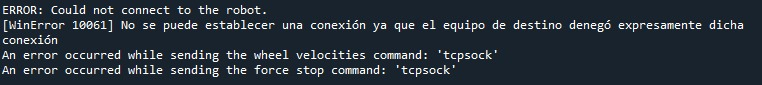
\includegraphics[width=0.8\textwidth]{error_conexion.png}
	\caption{Error de conexión con Pololu 3Pi+.}
	\label{fig:error_conexion}
\end{figure}

\subsection{Calibración de marcadores}
Una vez lograda la conexión con los Pololu 3Pi+, se tuvo que realizar una nueva calibración de los marcadores del OptiTrack para obtener el desfase del ángulo \textit{bearing} de cada marcador. Estos desfases son diferentes en cada marcador y se producen por la forma en que el OptiTrack identifica cada uno según la posición de sus esferas reflectivas.

En la fase anterior, se realizó una calibración con los marcadores del $1$ al $15$, sin embargo, se agregaron nuevos marcadores por lo que ahora se cuenta con $22$ de ellos para utilizar, de los cuales están inhabilitados el $1$ y $9$ ya que serán utilizados en otros proyectos de graduación. Por tanto, ahora se tienen disponibles los marcadores de la Figura \ref{fig:marcadores_disponibles}.

\begin{figure}[H]
	\centering
	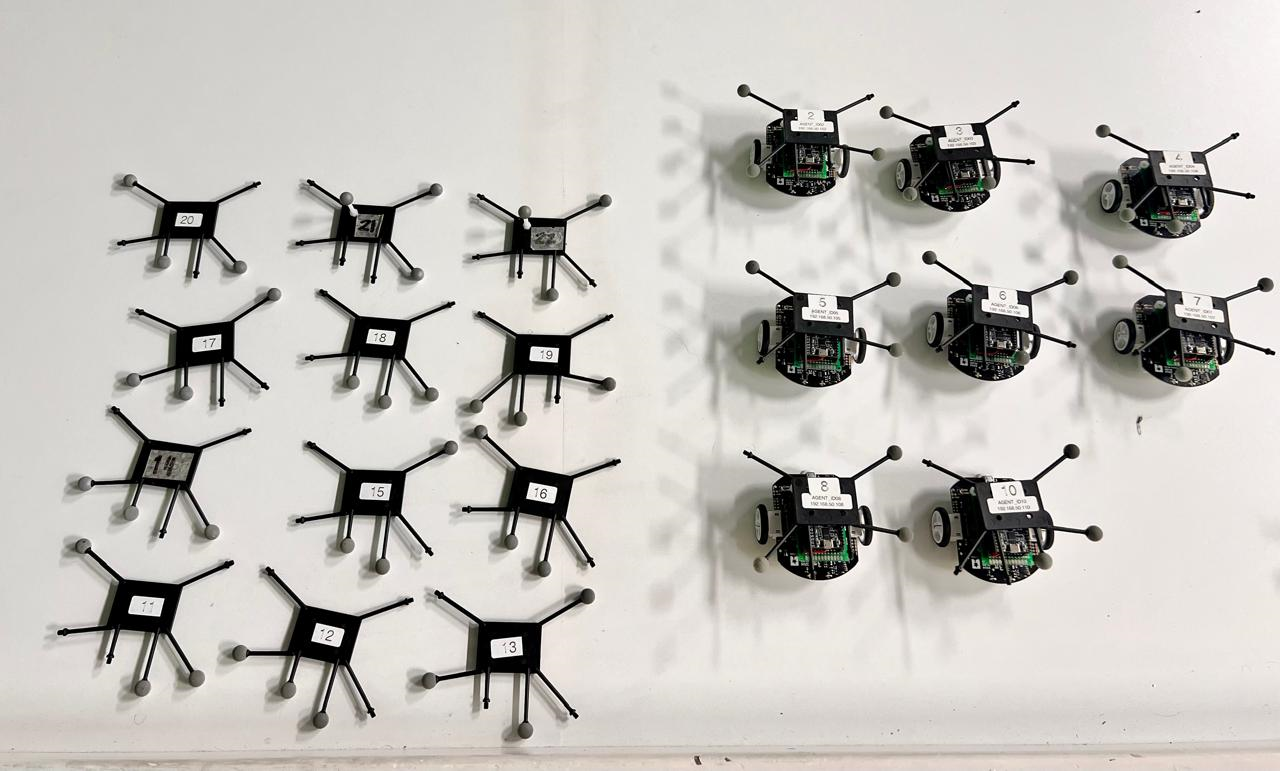
\includegraphics[width=0.8\textwidth]{marcadores_disponibles.png}
	\caption{Marcadores del OptiTrack disponibles para su uso.}
	\label{fig:marcadores_disponibles}
\end{figure}

Para corregir el desfase de cada marcador, se obtiene la orientación con ángulos de Euler en la secuencia $zyx$, luego, al primer ángulo que representa la rotación respecto al eje $z$ se le resta el desfase obtenido $\theta_z$.

Para realizar la calibración, se colocaron todos los marcadores disponibles de la Figura \ref{fig:marcadores_disponibles} con la misma orientación sobre el eje $y$ tal como se observa en la Figura \ref{fig:marcadores_calibracion}

\begin{figure}[H]
	\centering
	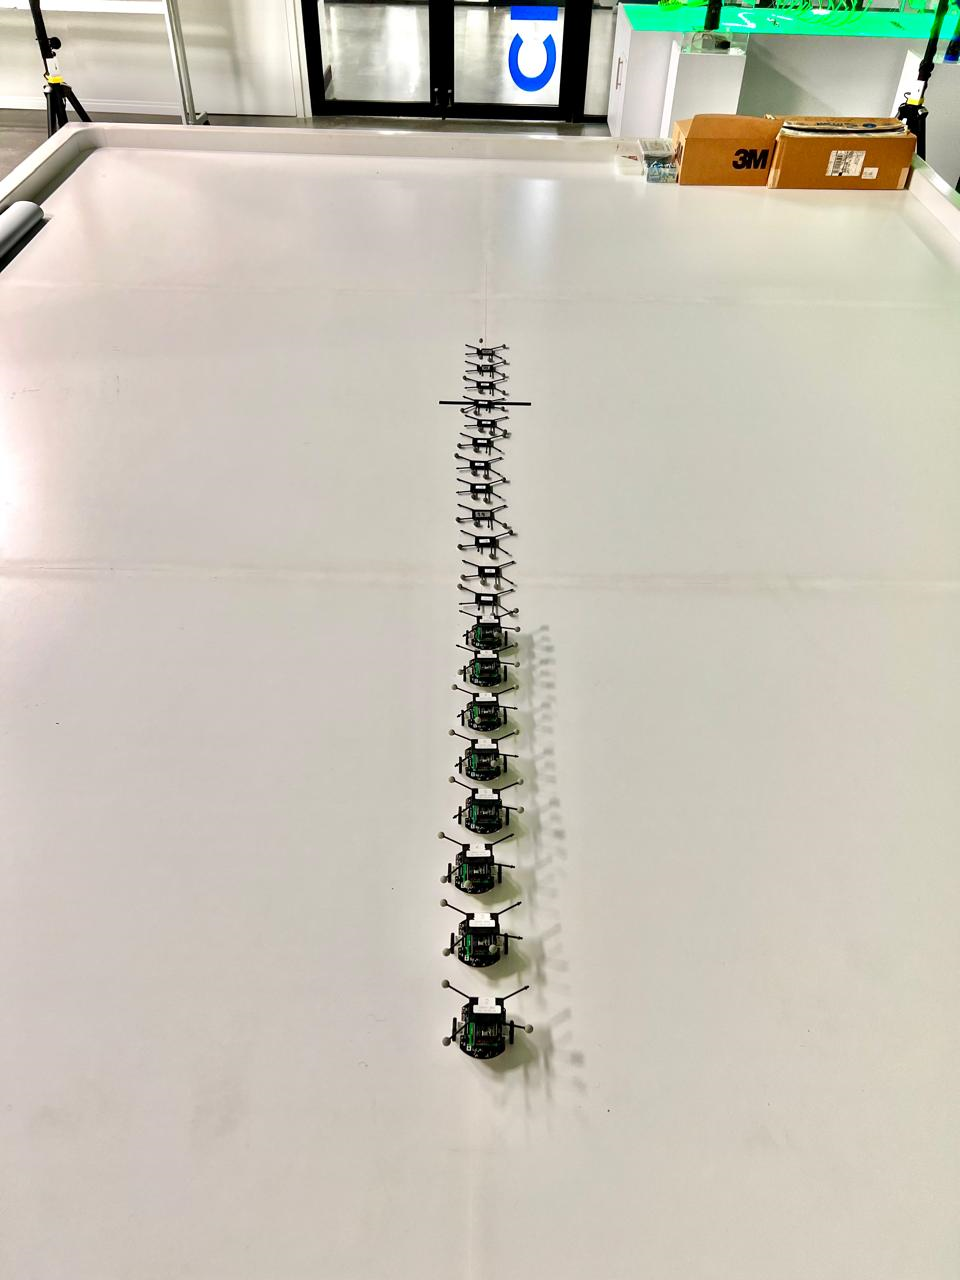
\includegraphics[width=0.8\textwidth]{marcadores_ejey.png}
	\caption{Marcadores alineados sobre el eje $y$ para calibración.}
	\label{fig:marcadores_calibracion}
\end{figure}

Al obtener la pose de cada marcador, se realizó la conversión a ángulos de Euler en la secuencia $zyx$ y se obtuvo los ángulos de desfase del Cuadro \ref{cuadro:desfases_iniciales}.

\begin{table}[H]
	\centering
	\begin{tabular}{|l|l|}
		\hline
		\textbf{Marcador} & \textbf{Desfase  $\theta_z$ en grados} \\ \hline
		2 & -47.2746822 \\ \hline
		3 & -90.32278167 \\ \hline
		4 & -135.7890952 \\ \hline
		5 & 179.3715195 \\ \hline
		6 & -141.0274548 \\ \hline
		7 & -175.0541793 \\ \hline
		8 & -78.11543097 \\ \hline
		10 & 143.2079276 \\ \hline
		11 & 111.0832797 \\ \hline
		12 & 166.1718189 \\ \hline
		13 & -127.3111755 \\ \hline
		14 & -109.4993486 \\ \hline
		15 & -40.73944282 \\ \hline
		16 & -104.1691129 \\ \hline
		17 & -121.1927571 \\ \hline
		18 & -92.48122033 \\ \hline
		19 & 4.298050244 \\ \hline
		20 & -133.2161012 \\ \hline
		21 & -112.0477043 \\ \hline
		22 & -15.28469666 \\ \hline
	\end{tabular}
	\caption{Desfases de marcadores disponibles alineados con el eye $y$.}
	\label{cuadro:desfases_iniciales}
\end{table}

Al comparar los desfases actuales con los obtenidos en la fase previa mostrados en el Cuadro \ref{cuadro:desfases_anteriores}, se observó que los valores son similares por lo que se optó tomar los desfases anteriores para los marcadores $1$ y $9$ faltantes en la calibración actual.

\begin{table}[H]
	\centering
	\begin{tabular}{|l|l|}
		\hline
		\textbf{Marcador} & \textbf{Desfase $\theta _{z}$ en grados} \\ \hline
		1                 & 91.99470274710572                      \\ \hline
		2                 & -46.814569482191594                    \\ \hline
		3                 & -92.39049071644509                     \\ \hline
		4                 & -138.20668559103328                    \\ \hline
		5                 & 176.37515477240987                     \\ \hline
		6                 & -144.1821533175259                     \\ \hline
		7                 & -176.31925348204803                    \\ \hline
		8                 & -79.95245389000435                     \\ \hline
		9                 & -9.87621045801094                      \\ \hline
		10                & 139.3578557303511                      \\ \hline
		11                & 111.93284607034238                     \\ \hline
		12                & 167.57610128913143                     \\ \hline
		13                & -128.0708601137765                     \\ \hline
		14                & -111.1403638963379                     \\ \hline
		15                & -43.41121657780576                     \\ \hline
	\end{tabular}
	\caption{Desfases de marcadores obtenidos en la fase previa.}
	\label{cuadro:desfases_anteriores}
\end{table}

Finalmente, en el Cuadro \ref{cuadro:desfases_finales} se observan los desfases finales para cada uno de los marcadores del $1$ al $22$. Estos valores se guardaron en un archivo .npy para aplicarlos luego de obtener la pose de cada marcador en el algoritmo y así tener siempre un ángulo respecto del eje $z$ igual a cero ($\theta_z$ = 0).

\begin{table}[!ht]
	\centering
	\begin{tabular}{|l|l|}
		\hline
		\textbf{Marcador} & \textbf{Desfase $\theta_z$ en grados} \\ \hline
		1 & 91.99470275 \\ \hline
		2 & -47.2746822 \\ \hline
		3 & -90.32278167 \\ \hline
		4 & -135.7890952 \\ \hline
		5 & 179.3715195 \\ \hline
		6 & -141.0274548 \\ \hline
		7 & -175.0541793 \\ \hline
		8 & -78.11543097 \\ \hline
		9 & -9.876210458 \\ \hline
		10 & 143.2079276 \\ \hline
		11 & 111.0832797 \\ \hline
		12 & 166.1718189 \\ \hline
		13 & -127.3111755 \\ \hline
		14 & -109.4993486 \\ \hline
		15 & -40.73944282 \\ \hline
		16 & -104.1691129 \\ \hline
		17 & -121.1927571 \\ \hline
		18 & -92.48122033 \\ \hline
		19 & 4.298050244 \\ \hline
		20 & -133.2161012 \\ \hline
		21 & -112.0477043 \\ \hline
		22 & -15.28469666 \\ \hline
	\end{tabular}
	\caption{Desfases para calibración de marcadores del $1$ al $22$.}
	\label{cuadro:desfases_finales}
\end{table}

\subsection{Selección de marcadores a utilizar}
Anteriormente, para obtener las poses de los marcadores se utilizaba una lista predeterminada con los valores enteros del $1$ al $12$ que serían los marcadores a utilizar. Sin embargo esto ocasionaba los siguientes problemas:

Para obtener las poses de los marcadores, la función \textit{robotat\_get\_pose} recibe como argumentos el objeto TCP y los números de marcadores. Al tener una lista predeterminada de valores, siempre se está solicitando la pose de los $12$ marcadores aunque no todos estén en uso, resultando en una solicitud de datos innecesaria para el servidor.

Además, dado que actualmente no se tienen disponibles los marcadores $1$ y $9$, se excede el \textit{Time Out} (tiempo de espera) para obtención de poses, lo que resulta en tiempos muertos durante la ejecución del código.

Por otro lado, para asignar los marcadores de cada agente, se debía elegir un intervalo  de valores consecutivos dentro de la lista predeterminada. Esto era problemático ya que limita a utilizar los agentes únicamente dentro del intervalo seleccionado, por lo que si un agente se descargaba, era obligatorio reemplazar las baterías para volver a utilizarlo



\subsection{Cálculo de velocidades de cada agente}
	Se cambió el signo de velocidad
	Se cambió el signo del peso en la etapa 3
	Se cambió el signo de velocidad en la etapa 0


\chapter{Optimización del algoritmo y su implementación}

\section{Limpieza de código y eliminación de funciones y variables obsoletas}
\section{Obtención de poses del Robotat}
	Ahora solo se pide la pose de los agentes a utilizar, antes se pedían todos los marcadores
\section{Posición de cada agente según el grafo de formación}
	Ahora los agentes siempre inician en la posición 0 del grafo de formación
\section{Implementación de operaciones matriciales con NumPy}
\subsection{Aplicar desfases de los marcadores}
\subsection{Cálculo de la distancia entre agentes}
\subsection{Cálculo del error de formación}

\section{Implementación de paralelismo computacional}





